%!TEX program = xelatex
%Template created by: Maciej Byczko
\documentclass[a4paper,12pt]{extarticle}  %typ dokumentu

% \usepackage[utf8]{inputenc} %rodzaj czcionki w dokumencie
\usepackage{geometry} %poprawienie marginesów
\usepackage{polski} %polskie znaki
\usepackage{multirow} %tabela
\usepackage{graphicx} %tabela
\usepackage{float} %poprawienie pozycji
\usepackage{fancyhdr} % header i footer
\usepackage{karnaugh-map} % rysowanie siatek karnaugh
\usepackage{hyperref} %tworzenie odnośników, \url{<url>}, \href{<file path, link>}{<text with link>} \pageref{}
\usepackage{amsmath} % Matma
\usepackage{boldline}%edytowanie grubości krawędzi w tabelach \hlineB{} \clineB{}{}
\usepackage{array}%grubsze kolumny w tabeli
\usepackage{bigstrut}
\usepackage{caption}
\usepackage{listings} %pisanie kodu w ładny sposób, begin{listings}[language=<język>]...end{listings} tak samo jak nazwa paczki
\usepackage{subcaption}

%Ustawienie paczki hyperref
\hypersetup{
     colorlinks,
     citecolor=black,
     filecolor=black,
     linkcolor=black,
     urlcolor=black
}

\definecolor{backcolour}{rgb}{0.95,0.95,0.92}
\definecolor{AO}{rgb}{0,0.5,0}
\definecolor{ZeroBlue}{rgb}{0,0.28,0.73}
\definecolor{DarkRed}{rgb}{0.85,0.16,0.16}

\lstset{
breaklines=true,
language=vhdl,
numbers=left,
tabsize=2,
numberstyle=\tiny,
backgroundcolor=\color{backcolour},
breakatwhitespace=false,
showspaces=false,                
showstringspaces=false,
showtabs=false,
commentstyle=\color{gray},
keywordstyle=\color{ZeroBlue},
% keywordstyle={[2]\color{DarkRed}},
% keywordstyle={[3]\color{ZeroBlue}},
}
\graphicspath{{pictures/}}
\geometry{margin=0.7in}
\pagestyle{fancy}

\cfoot{Strona \thepage}
\rhead{Strona \thepage}
\lhead{\typdoc}
\newcolumntype{?}{!{\vrule width 1.5pt}}

\title{\tytul}
\author{\tworcy}
\date{\data}

%-----------------------PRZYDATNE LINKI----------------------------------
%link do tworzenia tabeli https://tablesgenerator.com
%symbole matematyczne: https://oeis.org/wiki/List_of_LaTeX_mathematical_symbols
%narzędzia matematyczne: https://en.wikibooks.org/wiki/LaTeX/Mathematics
%krótkie podpowiedzi http://www.mif.pg.gda.pl/homepages/sylas/students/wdi/doc/latex-sciaga.html
%symbole do schematów: http://texdoc.net/texmf-dist/doc/latex/circuitikz/circuitikzmanual.pdf
%----------------------------------------------------------------------

%-----------------------SEKCJA DANYCH----------------------------------
\def\tytul{Licznik synchroniczny sterowany - FPGA} %<<< tytuł ćwiczenia
\def\nrcw{7} %<<< numer ćwiczenia
\def\data{10 Stycznia 2022r.} %<< data wykonania
\def\prowadzacy{dr inż. Jacek Mazurkiewicz} %<<<prowadzący
\def\nrgrupy{B} %<<<numer grupy
\def\tworcy{Maciej Byczko\\Bartosz Matysiak} %<<< autorzy
\def\zajinfo{PN 10:50 TP} %<<< informacje dotyczące zajęć
\def\typdoc{Sprawozdanie} %<<< typ dokumentu tj Sprawozdanie, zadania itp. {Matematyka dyskretna/Sprawozdanie z Miernictwa}
\begin{document}
\setlength{\headheight}{15pt}

\newcommand{\ov}[1]{\overline{#1} \ }

%-------------------------------------TABELA-DANYCH--------------------------------------------------
\begin{table}[H]
	\centering
	\resizebox{\textwidth}{!}{
		\begin{tabular}{|c|c|c|}\hline
			\begin{tabular}[c]{@{}c@{}}                     \tworcy     \end{tabular} &
			\begin{tabular}[c]{@{}c@{}}Prowadzący:\\        \prowadzacy \end{tabular} &
			\begin{tabular}[c]{@{}c@{}}Numer ćwiczenia\\    \nrcw       \end{tabular}          \\ \hline
			\begin{tabular}[c]{@{}c@{}}                     \zajinfo    \end{tabular} &
			\begin{tabular}[c]{@{}c@{}}Temat ćwiczenia:\\   \tytul      \end{tabular} & Ocena: \\ \hline
			\begin{tabular}[c]{@{}c@{}}Grupa:\\          \nrgrupy    \end{tabular}    &
			\begin{tabular}[c]{@{}c@{}}Data wykonania:\\    \data       \end{tabular} &        \\ \hline
		\end{tabular}}
\end{table}
%----------------------------------------------------------------------------------------------------
\tableofcontents
\cleardoublepage
% \section{Zadanie 1}
\section{Polecenie}
Licznik synchroniczny rewersyjny 8-bitowy pracujący w kodzie naturalnym binarnym. Wartość inicjująca licznik ma być ładowana z klawiatury komputera PC poprzez uruchomiony na nim terminal. Można także użyć klawiatury PS/2 - uwaga na inne wartości podawane przez klawiaturę - kody skaningowe - oraz inny moduł wejściowy do obsługi portu PS/2.

Oznacza to, że do przystawki dotrze kod naciśniętego klawisza poprzez port szeregowy RS232 lub port PS/2 i ten właśnie kod ma inicjować licznik. Licznik po przyjęciu kodu zaczyna liczyć - grupa wybiera czy będzie zwiększał swój stan - będzie początkowo - pozytywny, czy też zmniejszał swój stan - będzie początkowo - negatywny.

Bieżący stan licznika ma być wyświetlany na wyświetlaczu LCD w dowolnej, ale jednoznacznej i komunikatywnej formie. W dowolnym momencie pracy licznika możemy zmieniać kierunek zliczania wybranym guzikiem z przystawki. Może to być jeden guzik - przełącznik góra/dół, mogą być użyte dwa guziki - jeden włącza zliczanie w górę, drugi - zliczanie w dół.

Realizacja zadania wymaga zatem napisania w VHDL-u własnego modułu, który będzie realizował działanie licznika oraz spięcie tego modułu z gotowymi modułami obsługi urządzeń wejścia/wyjścia przystawki: odbiornika portu RS232 lub portu PS/2 oraz obsługi wyświetlacza LCD stanowiącego integralną część przystawki Spartan FPGA. 
\section{Rozwiązanie}
Projekt licznika się nie zmienia względem poprzednich zajęć, więc dla przypomnienia:

aby wykonać w pełni działający licznik wiemy że potrzebujemy następujące wejścia/wyjścia:
\begin{itemize}
	\item Wejście na parametry podane z klawiatury
	\item Zegar na podstawie którego wywołamy kolejny stan
	\item Reset za pomocą którego będziemy informować licznik że chcemy wprowadzić nową wartość
	\item Kontrolę w jaki sposób licznik będzie liczyć (do przodu/do tyłu)
\end{itemize}
Licznik bazuje na 8 bitach więc w momencie przepełnienia ustawiliśmy że licznik wraca do wartości:
\begin{itemize}
	\item Zerowej gdy liczy do przodu
	\item Maksymalnej gdy liczy do tyłu
\end{itemize}
Jedyna różnica w kodzie jest taka, że Spartan posiada zegar ze znacznie większą częstotliwością, więc na podstawie wykonania działania:

$$1Mhz = 10^6 Hz \rightarrow 50Mhz = 5*10^7Hz$$

$$\log_2(5*10^7Hz)\approx25.57$$

$$\frac{5*10^7Hz}{2^{25}}\approx1.49Hz$$

Dzięki tym obliczeniom wiemy, że musimy zastosować 25 bitowy dzielnik aby uzyskać częstotliwość w przybliżeniu $1Hz$.
\subsection{Kod VHDL}
\lstinputlisting{zadanie1/mainModule.vhd}
\subsection{Kod VHDL TestBench}
\lstinputlisting{zadanie1/counter_testbench.vhd}

\subsection{Symulacja}
\begin{figure}[H]
   \centering
   \caption{Początek symulacji}
   \resizebox*{\textwidth}{!}{
	  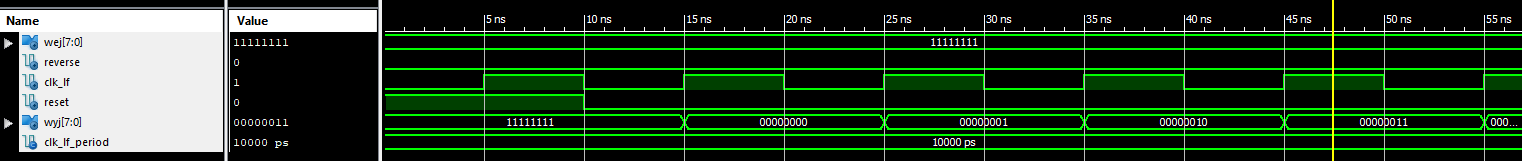
\includegraphics{zadanie1/simulation_run_1.png}
   }
\end{figure}
\begin{figure}[H]
	\centering
	\caption{Wprowadzenie nowej wartości}
	\resizebox*{\textwidth}{!}{
	   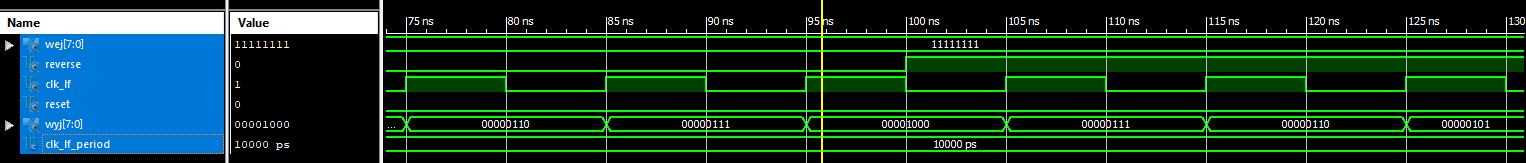
\includegraphics{zadanie1/simulation_run_2.png}
	}
 \end{figure}
 \begin{figure}[H]
	\centering
	\caption{Odwrócenie kolejności odliczania}
	\resizebox*{\textwidth}{!}{
	   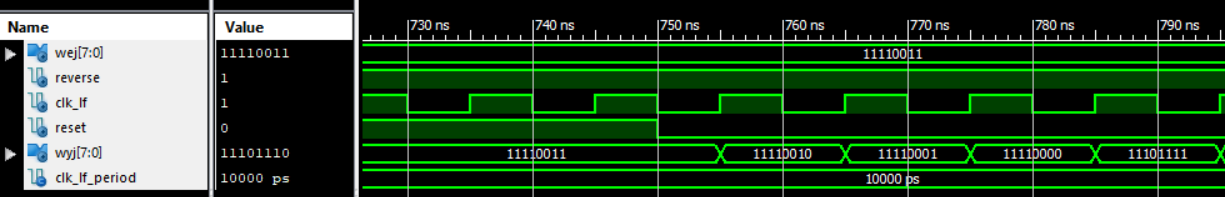
\includegraphics{zadanie1/simulation_run_3.png}
	}
 \end{figure}
 \subsection{Schemat układu z wykorzystaniem zaprojektowanego modułu}
 \begin{figure}[H]
	 \centering
	 \caption{Schemat z podłączoną klawiaturą oraz wyświetlaczem LED}
	 \resizebox*{\textwidth}{!}{
		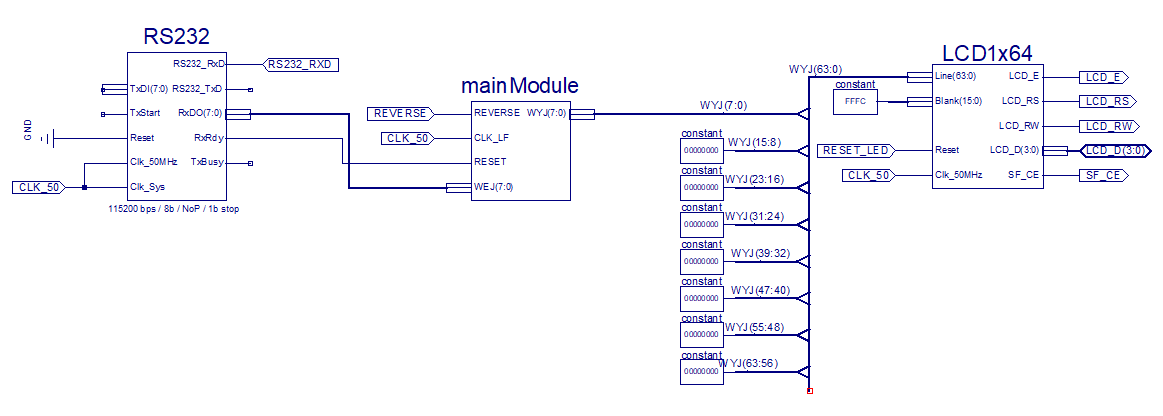
\includegraphics{zadanie1/scheme.png}
	 }
  \end{figure}
\section{Fizyczna implementacja}
\subsection{Kod UCF}
Normalnie Kod byłby w dwóch plikach:
GenIO.ucf oraz LDC.ucf lecz w celu poprawienia czytelności kody zostały umieszczone w jednym bloku 
\lstinputlisting{zadanie1/Combined.ucf}

\section{Wnioski}
Niestety przez zajęcia zdalne nie mieliśmy możliwości przetestowania zaprojektowanego układu.
Podczas wykonywania zadania pamiętaliśmy że przy włączonym dzielniku częstotliwości rezultaty na symulacji nie byłyby widoczne dlatego 
podczas symulacji wykomentowaliśmy część odpowiadającą za dzielenie.

Moduły wykorzystane w schemacie od Spartana nie różniły się znacznie od modułów ZL-9572 dzięki czemu nie było z nimi problemów.
\end{document}